\section{Visualization} 
\label{sec:visualization}

Continuing from the progress in the third milestone, we carried forward with the implementation of the chosen visualization design. This involved a number of steps that were carried out over the course of three weeks that resulted in the below visualization that now forms the basis of our progress. The contributions made in service of this visualization design are explained in separate subsections below.

\subsection{Design View}
\label{sec:design view}
Our visualization has a geographical map which represents the Los Angeles City based on the longitude and latitude values our data has provided. On the first glance of our visualization, you find many circles on the map and on hovering over a particular circle we get the number of bikes rented from that station. We have a histogram below the map which indicates the number of bikes that has been rented throughout the whole lifetime of the Metro Bike Share. We have provided a click function on the histogram which can be used to select a particular time-frame and related data from that time frame is reflected on the map.
\subsection{Supported User Interactions}
\label{sec:user interactions}
Our visualization design currently supports a number of interactions. These visualizations have been presented in the short movie as well. The following interactions are available to the user:
\begin{itemize}
    \item \textbf{Panning and Zooming}: The geographic map can be panned sideways to move around and locate different data points around the city. Also, the map can be zoomed in and out. Zooming in allows users to get a closer look into the data points on a street-level view. This way the bike stations look more distinguishable from one another. The zoom feature here is constrained and semantic in nature. This interaction follows the Shneiderman's mantra of having an overview first and then allowing to zoom in and filter data.
    \item \textbf{Pop-up Effect}: The individual data points support a "Hover Over" feature. Every time a data point i.e. a circle is hovered over, the color of the circle changes to blue with a more defined stroke around the circle. This makes the data point more visible and allows it to stand out, especially when there are a large number of similar data points around it. We decided on choosing the "Hover Over" action to show the effect rather than the "Click On" action since hovering over an element to have a detailed overview of a single data point is more effective and less time-consuming than clicking on it. Either way, this follows the Shneiderman's Detail-on-Demand task taxonomy.
    \item \textbf{Tooltip}: In addition to the "Hover Over" feature changing the color of the circle, a tooltip will also appear on top of each data point. Currently, this tooltip shows the number of bike pickups for a given location.
    \item \textbf{Histogram}: We have a histogram time frame at the bottom of the visualization window which indicates the number of bikes shared in each month based on the number of trips and passes issued. This histogram will stretch the width of the window. 
    \item \textbf{Click and Filter}: We have an 'Clikc On' feature on the histogram which allows users to filter data in the map based on the time-frame selection. Suppose the user wants to filter the data for a duration of any particular month, he needs to click on the rectangle representing that month of a year and the map will refresh and give the related data for the specified date.
\end{itemize}


\subsection{Design choices and rationale behind them}
\label{sec:design choices and rationale}

We went through good brainstorming sessions while discussing the design choices. Our common question was how do we visualize data that is as large as ours? 
We applied principles learned in our data visualization class which helped us a lot in finalizing the visualization so far. We derived new data which matches our tasks (listed in Task Abstraction section) to represent our visualization, we reduced and aggregated the data at hand to indicate total number of the bikes rented, we have added the interactions to change the view of data over time, we have faceted or partitioned our data using "Click On" operations so that a specific time-frame can be selected. 

\begin{itemize}
	\item \textbf{Geographical Map}: We made a choice to display the geographical map of Los Angeles because location is an important part of the meaning we’re trying to discover and the story we’re trying to tell. The X-axis represents the longitude and Y-axis represents the latitude information. We can associate stations with the highest number of bikes available. We have used map with certain navigation constraints like limiting bounds of pan, zoom, or rotation and while panning it doesn't pan off sides of the image, it doesn't zoom into an empty frame, and when rotating we can maintain the orientation of the viewpoint. When panning or zooming we are able to change the viewpoint.
		\begin{figure}[h]
		\centering % avoid the use of \begin{center}...\end{center} and use \centering instead (more compact)
		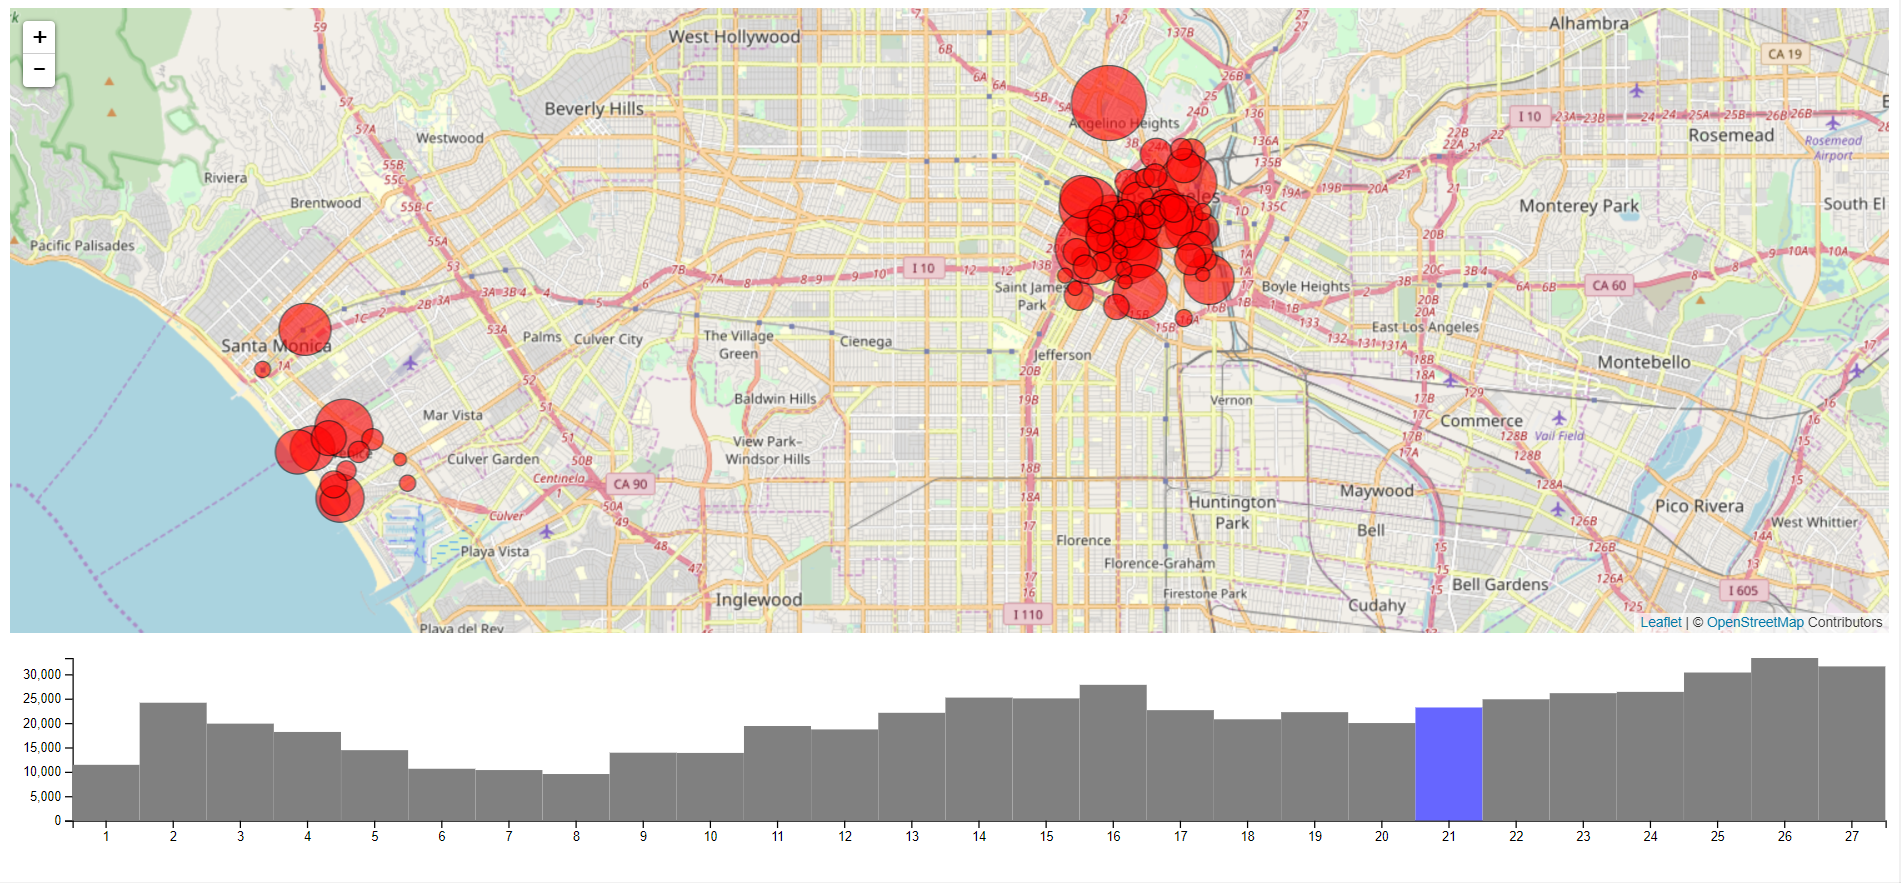
\includegraphics[scale=0.20]{figs/high_level.png}
		\caption{\footnotesize{High level overview of visualization}}
		\label{fig:First viz Chart}
		\captionsetup{justification=centering,margin=1cm}
		\vspace{-10pt}
	\end{figure}
	\item \textbf{Points and circles}: The data is discrete in our case so the marks are points and areas. The map uses circles that vary in size to encode differences in value — the larger the area, the greater the value. Each circle represents a station and their sizes indicate the number of bikes rented at each station.
	\item \textbf{Selecting}: Initially, we had thought of displaying a time histogram which had cross-filter support to brush through a series of time periods but later finalized on implementing the "Click On" feature as clicks act as a form of selection to filter time periods and is also user-interactive. When showing focus, we have some way at hinting at the context often done by using multiple views, one for focus and one for context. Histogram view shows full dataset, click filters a smaller subset allowing fine details to be shown. The clicked frame on the histogram represents the query and is applied to the other map.  
	\item \textbf{Hovering on circles}: We had a choice between two selection types: clicking the circles or to hover over the circles for further information. We realized based on Munzner's information that clicking is a heavyweight interaction vs hovering which is a lightweight interaction. So we decided to go ahead with hovering over circles as it suits our purpose of the visualization more. In this case, we may make many fetch requests in the process of mouseover interaction, but it does not interfere with our purpose of communicating the value of that point.
	\begin{figure}[h]
		\centering % avoid the use of \begin{center}...\end{center} and use \centering instead (more compact)
		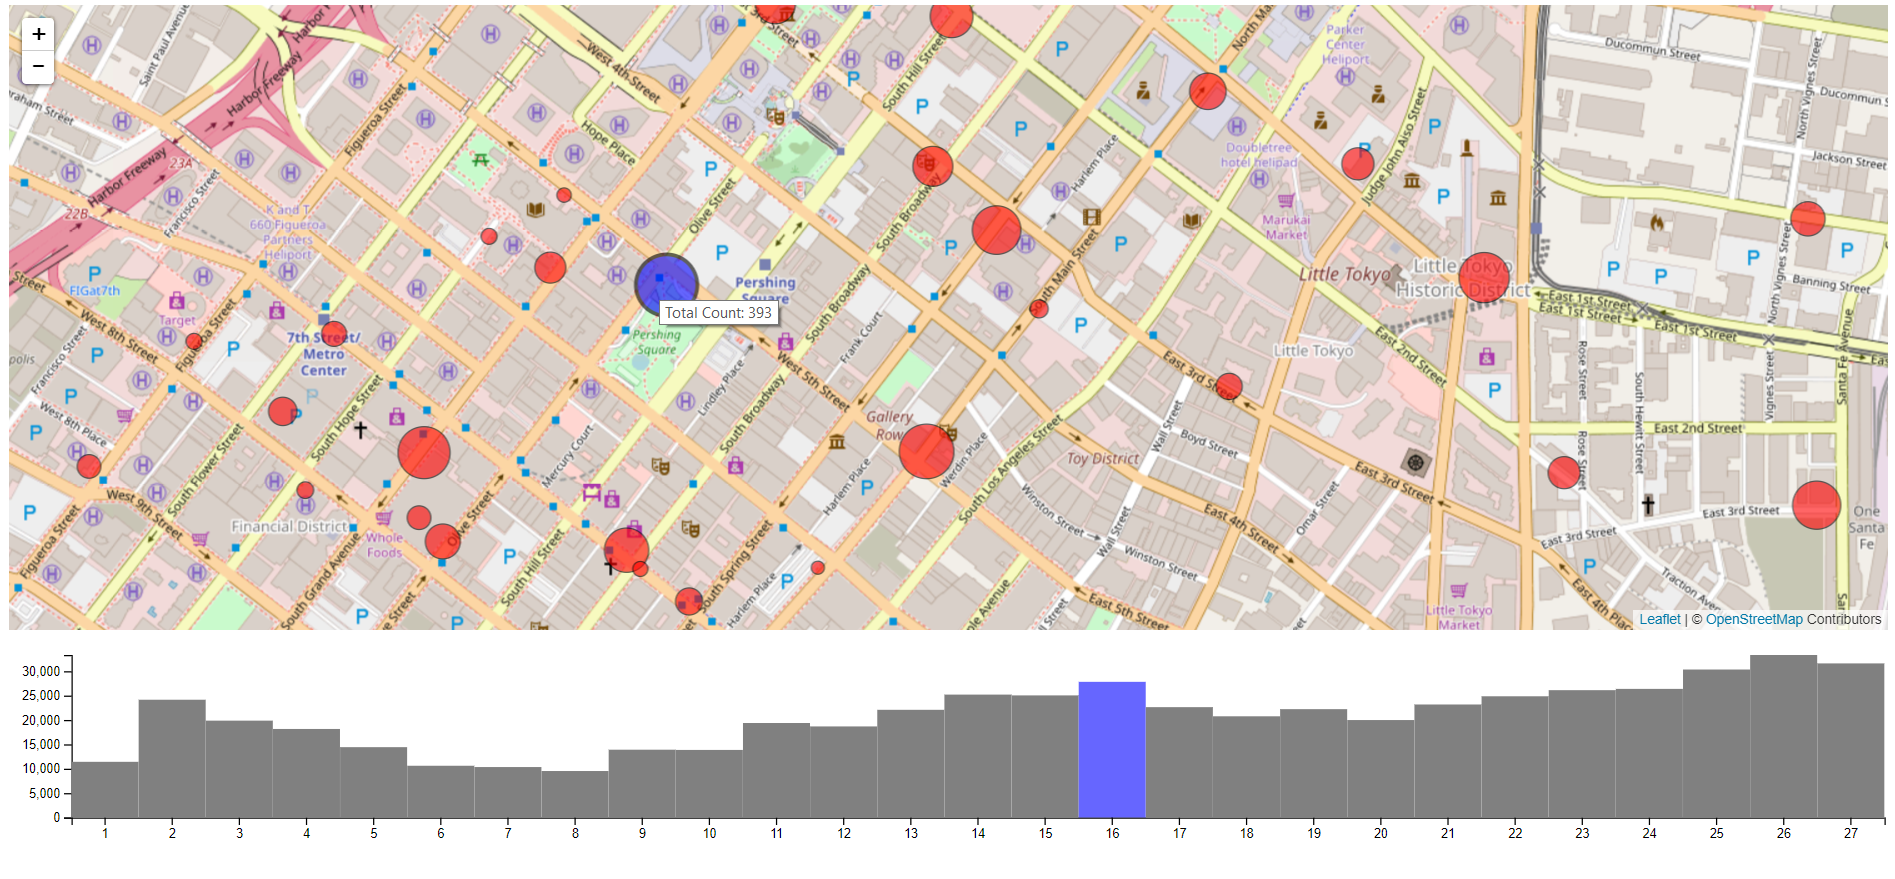
\includegraphics[scale=0.20]{figs/zoom_2.png}
		\caption{\footnotesize{Tooltip for individual data points}}
		\label{fig:First viz Chart}
		\captionsetup{justification=centering,margin=1cm}
		\vspace{-10pt}
	\end{figure}
	\item \textbf{Histogram}: Prior studies (Cleveland and McGill, Heer and Bostock) showed participants are more accurate in estimating the ratio between two bars when they are adjacent. Keeping this one and along with the application of Gestalt principles in our minds we chose histogram to represent the bike rent frequency as it is easier to compare and analyze between adjacent bar graphs.
		\begin{figure}[h]
		\centering % avoid the use of \begin{center}...\end{center} and use \centering instead (more compact)
		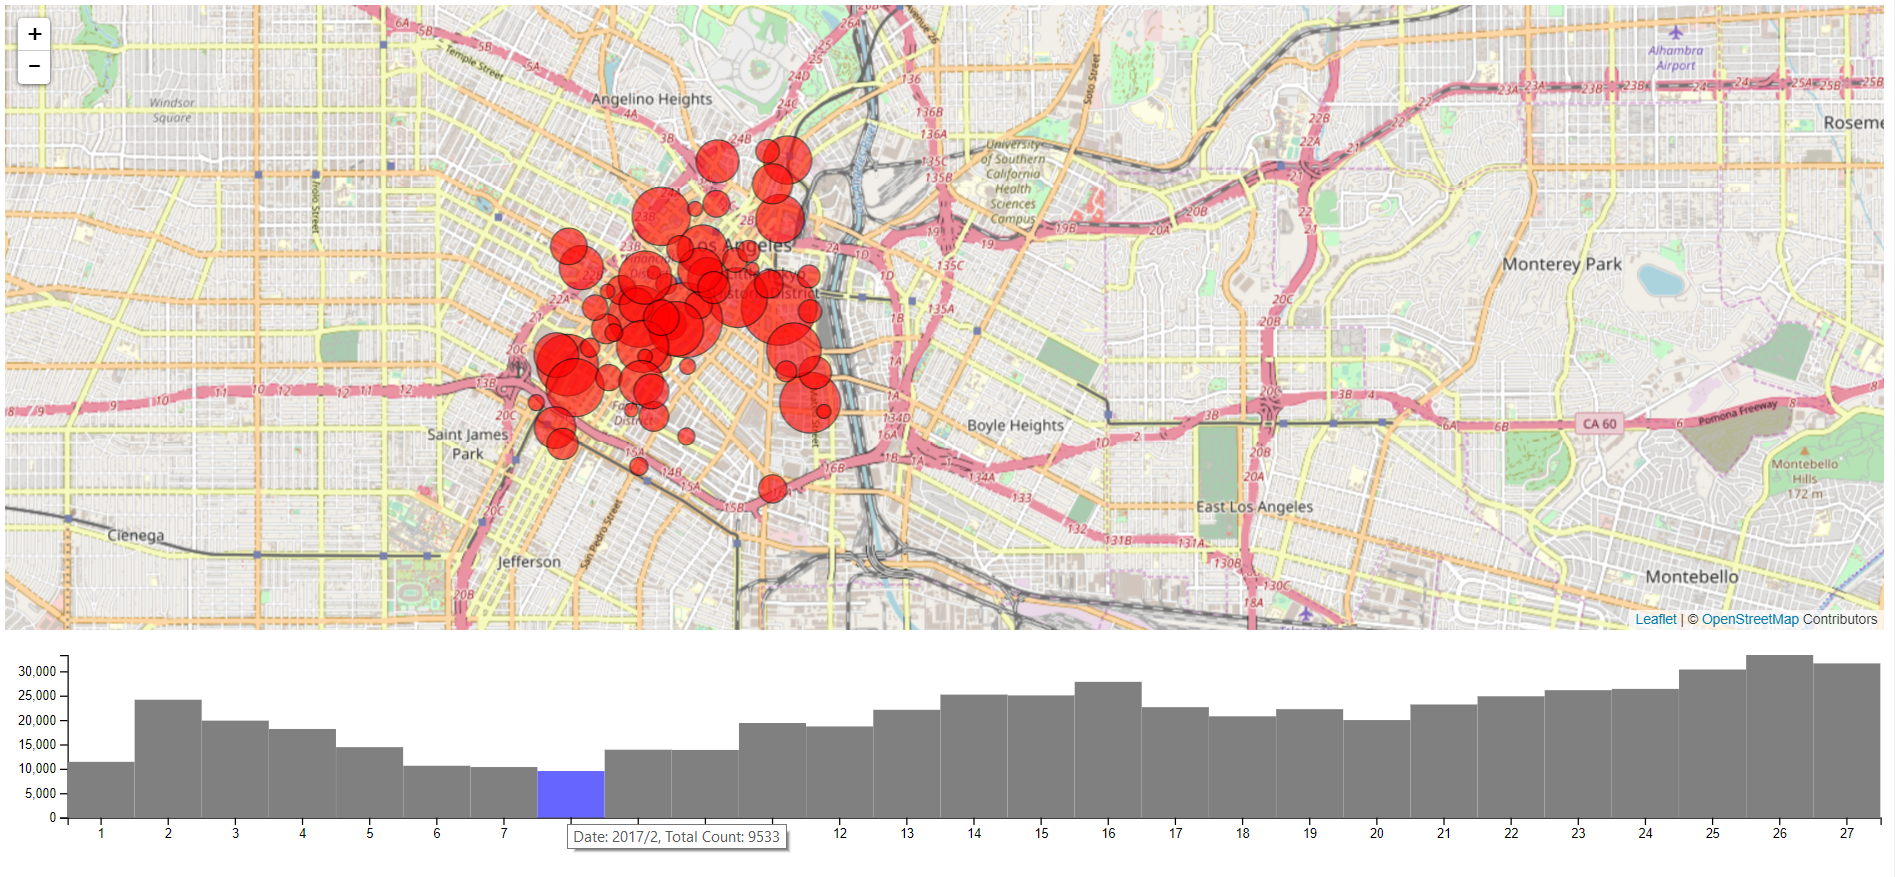
\includegraphics[scale=0.20]{figs/zoom.png}
		\caption{\footnotesize{Interaction support and tooltip for Histogram}}
		\label{fig:First viz Chart}
		\captionsetup{justification=centering,margin=1cm}
		\vspace{-10pt}
	\end{figure}
	\item \textbf{Color} : We chose warm saturated colors as saturation affects area perception. We made sure that the colors for data are darker or brighter than the other colors on the map so that the data will stand out more by pushing the map further into the background. Specially when using geographic maps for visualization, a host of different colors can appear on the background, be it foliage or buildings or offices. Our color choice had to stand out from these various colors and hence we chose colors that least blended in and were able to stand out in the map whilst not being overly saturated.
\end{itemize}


\subsection{Design relates to data and task abstractions}
\label{sec:design relates to abstractions}

\begin{itemize}
	\item Finding the trends - We were able to locate the busiest stations in Los Angeles Metro Area by the number of bikes available in a particular station indicated by the circle size in the map. The same encoding i.e. number of bike rents was used in the histogram but here it was plotted against time. We have met our Goal G1 and Task T1 mentioned in the Task Abstraction section thereby getting a mental picture of business according to location.
	\item Rental Histogram - We were able to find the total number of bikes rented each month based on the number of trips indicated by the histogram. We have met our Goal G1 and Task T2 mentioned in the Task Abstraction section thereby getting a mental picture of business according to location.
	\item Size of the circles on the map with "Click On" selection - This indicates the number of bikes available at that particular station in the selected time-frame. We have met our Task T2 which tells us how the volume of the rentals changes over time by filtering the data.
\end{itemize}


\subsection{Data and Task Analysis}
\label{sec:data and task abstraction}

We initially obtained our data from a popular online data source, Kaggle. The dataset was named \textit{Los Angeles Metro Bike Share Trip Data}. Even though this dataset had enough depth to reason about various trends and patterns, it was less in number which made us look for other sources of similar data. We then found a substantial amount of data in the Metro Bike Share database. Bike Share Metro is a bike sharing service providing in services in Downtown LA, Port of LA and Venice. This data seemed to fulfill our requirements for this project. This data, like the one before, is from \textit{Los Angeles} and contains the shared bike ride information for nearly 2.5 years, 2016 Q3 to 2018 Q3. 

The structure of the data sources provides the details of where and when journeys are made. In the below-mentioned data-sets we have four spatial attributes namely, start\_lon, start\_lat, end\_lon and end\_lat. The data-set has a total of 14 attributes and they are as follows: 

\begin{itemize}
    \item trip\_id - Unique ID for a particular trip - This is of type integer
    \item duration - Duration of the trip in minutes - This is of type integer
    \item start\_time - Start time of the trip - This is a timestamp in format mm/dd/yyyy hh:mm
    \item end\_time - End time of the trip - This is a timestamp in format mm/dd/yyyy hh:mm
    \item start\_lon - Starting position longitude - This is of type float
    \item start\_lat - Starting position latitude - This is of type float
    \item start\_station - The station ID where the trip originated - This is of type integer
    \item end\_station -  The station ID where the trip terminated - This is of type integer
    \item end\_lat - Destination latitude - This is of type float
    \item end\_lon - Destination longitude - This is of type float
    \item bike\_id - Id for each bike - This is of type integer
    \item plan\_duration - Duration of the customer's plan - This is of type integer
    \item passholder\_type - The name of the pass holder's plan like "One Day Pass" or "Monthly Pass" or "Walk-up" or "Flex Pass" - This is of type string
    \item trip\_route\_category\ -  "Round Trip" for trips starting and ending at the same station or "One Way" for all other trips - This is of type string
\end{itemize}

In order to create a new design process model for data visualization, we utilized our team’s combined experience in visualization design as well as the concepts from existing models as a guide to identify different stages and components of the process. As a redesign team, we identified the goals, and tasks employed in an iterative process for our own visualization project. 

In our first milestone, we understood the needs of bike share systems and identified the related data from Metro Bike share on which we could work on to identify the tasks. In our second milestone, we ideated several new designs by many discussions among ourselves to generate a plethora of concepts and then winnow these into good ideas to better visualize the bike share system. In our third milestone, we finalized upon a single visualization design which we decided to work on. This design incorporates various visualizations within a single frame that are layered in an interactive manner. These prototypes have been built to handle and visualize real data-sets, and it is common that, as prototypes get constructed, more design requirements or ideas may be explored and discovered, highlighting the iterative nature of visualization design. Another aspect of the making activity goes beyond design i.e. to employ software engineering and development techniques for writing code and programs to build visualizations to meet the needs of the users. We are using JavaScript together with D3.js and Leaflet to build and generate interactive visualizations. In the final milestone, we have the final design activity in the visualization framework i.e. the deploy activity, with the motivation to construct a visualization system and bring it into effective action in a real-world setting in order to support the goals. The overall visualization artifact of this activity is a usable visualization system. This activity is the ultimate goal of problem-driven visualization design since it supports real-world users in their own work environments. 

We applied Shneiderman's task taxonomy to further drill down on the tasks we needed to do. As per this taxonomy, we first get the overview of the data we have with us. Based on this our main focus is on the number of customers and the locations from which the bikes are rented. We zoom in on the tasks which interest us to analyze which places see the maximum number of business each day, and to see how the business is growing over time. We filter out the uninteresting data which is not of use in constructing the visualization (like bike station IDs). We can get more details-on-demand by first, panning and zooming into specific geographic locations in the map and then, hovering over data items in the map which bring up tooltips to display information specific to a location or a single bike ride. In this process, we can retrieve the data required for our analysis. By following the above taxonomy so far we could classify our goals into the following:

\begin{itemize}
    \item \textbf{G1}: Get a mental picture of business according to location:
    It will be very helpful in analyzing the viability of the bike share system if we could get a mental picture, around which geographic locations most of the business tend to gather. If there was a visible comparison between different locations, it would be so much easier to comprehend where the focus of the business should be, moreover if we can find some connection between high volume of the rentals at those locations, the same model could also be implemented in other locations with similar potential. The idea of business can be explained by the number of drop-offs and hires from a specific station. Typically, a station having a high number of hires has more business. For our visualization, we have mapped the number of hires from each station which gives a good measure of business and residence in a specific location.

    \item \textbf{G2}: How the volume of the rentals changes over time:
    We have visualized how the number of customers have changed over time which in turn provided us with clarifications about which time of the year people tend to chose this form of transport over others. That would be beneficial to understand what compels them to eschew bikes over the other time of the years and what steps could be taken to alleviate their discomfort.
 
\end{itemize}

To identify the smaller task in support of the goals, we can take the following steps.

\begin{itemize}
    \item \textbf{T1}: Getting the overview of the data: 
    First, we must identify all the stations from their longitude and latitude over the city of Los Angeles. This will give us an insight into how all the renting stations are spread over the city. And moreover, if there is a heavy density of stations in some particular locations, we can then analyze how well individual stations are performing in that heavy cluster and can come to decisions about whether some stations may be relocated in some other location where the density of the stations is relatively low.

    \item \textbf{T2}: Filtering Based Geographic Mapping:
    This visualization adds a dynamic element to the previous static visualization. We have mapped the number of bike hires in a per day, per month basis for a substantial span of time. The data is represented in the geographic plane and can be filtered by selecting different time ranges in the time histogram. This way we can get an analysis of the data from nearly 2.5 years which will give us clear insight into the growth/decline of the business model over time.

\end{itemize}

\subsection{Implementation}
\label{sec:implementation}

The technologies we used in our project are as follows:

\begin{itemize}
	\item \textbf{Programming Languages}:  JavaScript and Python. Javascript has been the primary language for our web development efforts. While HTML and CSS was used to form the outer skeleton and design of our interface, Javascript is the brains behind the visualization. In addition to this, Python was used in the initial data cleaning and scripting phase.\newline
	With our primary data being in a raw CSV format, we had to parse and clean it to make it more sensible and structured for further processing. This CSV format data was converted into GeoJSON in order to be ingested for map plotting and then into a Javascript array for further data manipulation.
	\item \textbf{Libraries}: D3 is a JavaScript library for visualizing data with HTML, SVG, and CSS. D3 has been the primary library that supported our visualization designs. D3 makes data visualizations incredibly easy and straightforward. Our time histogram and the geographic map was made using D3 along with the interaction between these two visualizations.\newline
	Leaflet is a widely used open source JavaScript library used to build web mapping applications. This library was used to generate the underlying geographic map of Los Angeles city. We chose this library over other options because of its lightweight, support for large number of interactions and extensive documentation on the web. Panning and zooming is an interaction feature courtesy of the Leaflet library.
	\item \textbf{Platform}: We have not used a stand-alone dedicated platform for our visualization but all of our visualization testing and debugging was done using Google Chrome. Chrome makes it easier for developers to debug errors and step through program execution in a very easy manner.
\end{itemize}

\textit{Summary}: We have completed our visualization as part of this milestone.